\documentclass[11pt,a4paper,openany]{report}

\usepackage{fontspec}
\usepackage[french]{babel}
\usepackage{newunicodechar}
\newunicodechar{→}{\ensuremath{\rightarrow}}
\newunicodechar{≥}{\ensuremath{\geq}}
\newunicodechar{≤}{\ensuremath{\leq}}
\usepackage{csquotes}
\usepackage{microtype}

\usepackage[a4paper,top=2.5cm,bottom=2.5cm,left=2.5cm,right=2.5cm,headheight=14pt]{geometry}
\usepackage[table]{xcolor}
\usepackage{graphicx}
\usepackage{pdflscape}
\usepackage{float}
\usepackage{booktabs}
\usepackage{tabularx}
\usepackage{xltabular}
\usepackage{array}
\usepackage{enumitem}
\usepackage{titlesec}
\usepackage{fancyhdr}
\usepackage{caption}
\usepackage{tikz}
\usetikzlibrary{positioning,arrows.meta}
\usepackage[most]{tcolorbox}
\usepackage{listings}
\usepackage{hyperref}

\graphicspath{{build/figures/}{captures/}{images/}}

\definecolor{primaire}{HTML}{1F3A5F}
\definecolor{secondaire}{HTML}{3C6E9F}
\definecolor{fondgris}{HTML}{F2F4F7}
\definecolor{alerte}{HTML}{B3261E}

\hypersetup{
  colorlinks=true,
  linkcolor=primaire,
  urlcolor=secondaire,
  pdftitle={Rapport de projet : Gestion d'une boutique en ligne},
  pdfauthor={LAHMOUZ Hamza, ELAOUAD Abdelhamid},
  pdfsubject={Module Architecture JEE, ENSA Agadir},
}

\titleformat{\chapter}[display]
  {\normalfont\color{primaire}}
  {\large\mdseries\scshape \chaptertitlename\ \thechapter}
  {4pt}
  {\Huge\bfseries\raggedright}
  [\vspace{4pt}{\color{secondaire}\titlerule[1.2pt]}]
\titlespacing*{\chapter}{0pt}{0pt}{24pt}
\titleformat{\section}{\Large\bfseries\color{primaire}}{\thesection}{0.8em}{}
\titleformat{\subsection}{\large\bfseries\color{secondaire}}{\thesubsection}{0.8em}{}
\titleformat{\paragraph}[runin]{\normalsize\bfseries\color{primaire}}{}{0pt}{}[ :]
\setcounter{secnumdepth}{2}
\setcounter{tocdepth}{1}

\pagestyle{fancy}
\fancyhf{}
\renewcommand{\chaptermark}[1]{\markboth{#1}{}}
\fancyhead[L]{\small\color{primaire}Gestion d'une boutique en ligne}
\fancyhead[R]{\small\nouppercase{\leftmark}}
\fancyfoot[L]{\small Projet Architecture JEE · ENSA Agadir}
\fancyfoot[R]{\small\thepage}
\renewcommand{\headrulewidth}{0.4pt}
\renewcommand{\footrulewidth}{0.4pt}
\fancypagestyle{plain}{%
  \fancyhf{}
  \fancyfoot[L]{\small Projet Architecture JEE · ENSA Agadir}
  \fancyfoot[R]{\small\thepage}
  \renewcommand{\headrulewidth}{0pt}
}

\setlength{\emergencystretch}{3em}
\setlist{itemsep=2pt,topsep=4pt}
\setlist[itemize]{label=\textbullet}
\captionsetup{font=small,labelfont={bf,color=primaire}}
\captionsetup[table]{position=top}
\renewcommand{\arraystretch}{1.25}
\newcolumntype{L}{>{\raggedright\arraybackslash}X}
\newcolumntype{P}[1]{>{\raggedright\arraybackslash}p{#1}}

\renewcommand{\lstlistingname}{Extrait}
\lstset{
  basicstyle=\ttfamily\fontsize{8}{9.8}\selectfont,
  keywordstyle=\bfseries\color{primaire},
  commentstyle=\itshape\color{black!55},
  stringstyle=\color{secondaire},
  breaklines=true, breakatwhitespace=false, breakindent=2em,
  columns=fullflexible, keepspaces=true, showstringspaces=false, tabsize=4,
  frame=single, rulecolor=\color{black!25}, backgroundcolor=\color{fondgris},
  xleftmargin=4pt, xrightmargin=4pt, framesep=4pt, aboveskip=8pt, belowskip=8pt,
  captionpos=b, extendedchars=true,
}

\newcommand{\code}[1]{\texttt{\NoAutoSpacing #1}}
\newcommand{\entete}[1]{\textbf{\color{white}#1}}
\newcommand{\ligneentete}{\rowcolor{primaire}}

\newcommand{\diagramme}[3]{%
  \begin{figure}[H]
    \centering
    \includegraphics[width=\linewidth,height=0.78\textheight,keepaspectratio]{#1}
    \caption{#2}\label{#3}
  \end{figure}}
\newcommand{\diagrammesuite}[4][0.74]{%
  \begin{figure}[H]
    \centering
    \includegraphics[width=\linewidth,height=#1\textheight,keepaspectratio]{#2}
    \caption{#3}\label{#4}
  \end{figure}}

\newcommand{\fichecas}[4]{%
  \par\noindent
  \begin{tabularx}{\linewidth}{>{\columncolor{fondgris}\bfseries}P{3.2cm}L}
    \toprule
    Acteur(s) & #1 \\
    Précondition & #2 \\
    Postcondition & #3 \\
    Règles & #4 \\
    \bottomrule
  \end{tabularx}\par\smallskip}
\newcommand{\scenario}[1]{\par\medskip\noindent{\bfseries\color{secondaire}#1}\par\nopagebreak}

\newtcolorbox{afaire}{colback=alerte!6,colframe=alerte,fonttitle=\bfseries,title=À compléter}

\newcommand{\capture}[2]{%
  \IfFileExists{captures/#1.png}{%
    \begin{figure}[H]
      \centering
      \includegraphics[width=0.92\linewidth,height=0.38\textheight,keepaspectratio]{captures/#1.png}
      \caption{#2}
    \end{figure}}{%
    \begin{afaire}#2 (fichier attendu : \code{captures/#1.png})\end{afaire}}}

\addto\captionsfrench{\def\tablename{Tableau}}

\begin{document}

\begin{titlepage}
  \newgeometry{top=2cm,bottom=2cm,left=2.2cm,right=2.2cm}
  \centering

  % Logos facultatifs : images/logo-uiz.png et images/logo-ensa.jpg
  \noindent
  \begin{minipage}[c]{0.22\linewidth}
    \IfFileExists{images/logo-uiz.png}{
\includegraphics[width=\linewidth]{images/logo-uiz.png}}{}
  \end{minipage}\hfill
  \begin{minipage}[c]{0.52\linewidth}
    \centering
    {\large\bfseries Université Ibn Zohr}\\[2pt]
    École Nationale des Sciences Appliquées\\
    d'Agadir
  \end{minipage}\hfill
  \begin{minipage}[c]{0.22\linewidth}
    \raggedleft
    \IfFileExists{images/logo-ensa.jpg}{
\includegraphics[width=\linewidth]{images/logo-ensa.jpg}}{}
  \end{minipage}

  \vspace{0.6cm}
  {\color{primaire}\rule{\linewidth}{0.6pt}}

  \vspace{2.2cm}
  {\Large\scshape Rapport de projet}\\[6pt]
  {\large Module : Architecture JEE · DLA2}

  \vspace{1.2cm}
  \begin{tcolorbox}[colback=fondgris,colframe=primaire,boxrule=1pt,arc=2pt,
                    left=10pt,right=10pt,top=14pt,bottom=14pt,halign=center]
    {\Huge\bfseries\color{primaire} Gestion d'une boutique en ligne}\\[10pt]
    {\large Application web Jakarta EE avec Servlets, JSP, JSTL et Hibernate}
  \end{tcolorbox}

  \vspace{1.6cm}
  {\small Catalogue · Panier en session · Commandes transactionnelles · Back-office d'administration}

  \vfill

  \noindent
  \begin{minipage}[t]{0.48\linewidth}
    \raggedright
    {\bfseries\color{primaire} Réalisé par :}\\[4pt]
    LAHMOUZ Hamza\\
    ELAOUAD Abdelhamid
  \end{minipage}\hfill
  \begin{minipage}[t]{0.48\linewidth}
    \raggedleft
    {\bfseries\color{primaire} Encadré par :}\\[4pt]
    Pr. BENIDER Zahra
  \end{minipage}

  \vspace{2cm}
  {\color{primaire}\rule{\linewidth}{0.6pt}}\\[4pt]
  Année universitaire 2026 – 2027
  \restoregeometry
\end{titlepage}


\pagenumbering{roman}
\tableofcontents
\listoffigures
\listoftables
\cleardoublepage
\pagenumbering{arabic}

\chapter{Introduction et contexte}

\section{Contexte}

Une petite boutique qui gère ses produits et ses commandes à la main (fichiers Excel, échanges
téléphoniques) s'expose à des erreurs de stock, à une mauvaise traçabilité des commandes et à une
visibilité limitée auprès de ses clients. Le projet consiste à lui fournir une application web de vente en
ligne : un catalogue public, un espace client (panier, commandes, historique, profil) et un back-office
d'administration.

\section{Problématique}

Comment offrir à une boutique un outil web simple permettant de publier un catalogue organisé par
catégories, de recevoir des commandes en ligne et d'en suivre le traitement, tout en garantissant la
cohérence des données (stock, prix, historique) ?

\section{Objectifs}

\begin{enumerate}
  \item Permettre aux visiteurs de consulter le catalogue et de rechercher des produits.
  \item Permettre aux clients authentifiés de gérer un panier et de passer des commandes.
  \item Permettre à l'administrateur de gérer les catégories, les produits, les commandes et les utilisateurs.
  \item Concevoir le système avec UML avant son implémentation.
  \item Mettre en œuvre une architecture MVC en Jakarta EE (Servlets, JSP, JSTL) avec Hibernate pour la persistance.
  \item Versionner le travail avec Git et GitHub (tickets, branches, pull requests).
\end{enumerate}

\section{Périmètre}

Le périmètre est celui du cahier des charges (§1.4). Sont \textbf{hors périmètre} : le paiement en ligne réel
(le paiement est simulé, à la livraison), la livraison et le suivi transporteur, la gestion multi-boutiques,
l'application mobile et l'envoi d'e-mails transactionnels.

\section{Acteurs}

\begin{table}[H]
  \centering\small
  \caption{Acteurs du système}
  \begin{tabularx}{\linewidth}{P{2.4cm}LL}
    \ligneentete
    \entete{Acteur} & \entete{Description} & \entete{Accès} \\
    Visiteur & Internaute non authentifié & Catalogue, recherche, fiche produit, inscription, connexion \\
    \midrule
    Client & Utilisateur connecté avec le rôle CLIENT ; hérite des droits du Visiteur & Panier, commandes, historique, profil \\
    \midrule
    Administrateur & Utilisateur connecté avec le rôle ADMIN & Back-office : catégories, produits, stock, commandes, utilisateurs, tableau de bord \\
    \bottomrule
  \end{tabularx}
\end{table}

\chapter{Processus de développement : modèle en Y}

\section{Principe}

Le projet suit le \textbf{modèle en Y} : un processus itératif, piloté par les cas d'utilisation, dans lequel la
capture des besoins fonctionnels et la capture des besoins techniques sont menées en parallèle avant de se
rejoindre dans la branche de conception et de réalisation (figure~\ref{fig:modele-y}).

\begin{figure}[H]
  \centering
  \begin{tikzpicture}[
      etape/.style={draw=primaire,fill=fondgris,rounded corners=3pt,thick,
                    align=center,text width=6.2cm,inner sep=7pt,font=\small},
      fleche/.style={-{Stealth[length=3mm]},thick,draw=secondaire}]
    \node[etape] (fonc) at (-3.8,0)
      {\textbf{Branche fonctionnelle}\\besoins, cas d'utilisation,\\classes du domaine};
    \node[etape] (tech) at (3.8,0)
      {\textbf{Branche technique}\\Java 17, Jakarta EE 10, Tomcat 10.1,\\Hibernate 6, MySQL 8, architecture MVC};
    \node[etape] (conc) at (0,-2.7)
      {\textbf{Conception préliminaire et détaillée}\\classes de conception, séquences};
    \node[etape] (real) at (0,-5.0)
      {\textbf{Codage, tests, déploiement (.war)}\\itérations successives,\\une branche par fonctionnalité};
    \draw[fleche] (fonc.south) -- (conc.north west);
    \draw[fleche] (tech.south) -- (conc.north east);
    \draw[fleche] (conc) -- (real);
  \end{tikzpicture}
  \caption{Le modèle en Y appliqué au projet}\label{fig:modele-y}
\end{figure}

\section{Branche fonctionnelle}

\begin{itemize}
  \item Rédaction du cahier des charges (\code{docs/cahier-des-charges.md}) : 23 besoins fonctionnels codés BF01 à BF23
        et priorisés (P1 indispensable, P2 important, P3 souhaitable), 16 règles de gestion RG01 à RG16,
        12 besoins non fonctionnels BNF01 à BNF12.
  \item Diagrammes de cas d'utilisation (Visiteur/Client et Administrateur), descriptions textuelles
        (chapitre~\ref{chap:cas}), diagramme de classes du domaine.
\end{itemize}

\section{Branche technique}

\begin{itemize}
  \item Technologies imposées par le module : Java 17, Jakarta EE 10 (Servlet 6.0, JSP 3.1, JSTL 3.0), Tomcat 10.1,
        Hibernate ORM 6, MySQL 8, Maven (packaging \code{war}), Bootstrap 5, jBCrypt, PlantUML.
  \item Architecture MVC N-tiers : navigateur, Tomcat (couches web et métier), serveur MySQL.
  \item Configuration Hibernate (\code{hibernate.cfg.xml}, génération des tables par \code{hbm2ddl.auto = update}) et
        configuration web (\code{web.xml} : session, encodage, pages d'erreur).
\end{itemize}

\section{Branche de conception et de réalisation}

\begin{itemize}
  \item Conception : diagrammes de classes de conception (couche web, couche métier) et diagrammes de séquence.
        Tous les diagrammes ont été versionnés avant la première ligne de code (commit \code{4fc0fac}), puis mis à jour
        au fil des itérations quand l'implémentation a précisé la conception (commits \code{docs:} des branches
        \code{feature/catalogue}, \code{feature/commande}, \code{feature/gestion-commandes}, \code{feature/p3} et
        \code{feature/coherence-finale}).
  \item Réalisation : une itération par groupe de fonctionnalités, chacune livrée sur une branche \code{feature/*},
        vérifiée par des tests manuels (navigateur et requêtes HTTP) puis fusionnée dans \code{main} par pull request.
\end{itemize}

\section{Itérations et suivi GitHub}

Le backlog est suivi dans \textbf{GitHub Issues} : un ticket par étape, avec la liste à cocher des codes BF/RG
concernés. Chaque étape est développée sur sa propre branche et fusionnée par une pull request dont la
description reprend les besoins couverts, les règles appliquées et les tests manuels effectués
(tableau~\ref{tab:iterations}).

\begin{table}[H]
  \centering\small
  \caption{Itérations (cahier des charges §8.3), tickets, branches et pull requests}\label{tab:iterations}
  \begin{tabularx}{\linewidth}{cLcP{4.5cm}c}
    \ligneentete
    \entete{It.} & \entete{Étape} & \entete{Ticket} & \entete{Branche} & \entete{PR} \\
    1 & Modélisation UML (cas d'utilisation, classes, séquences) & \#4 & \code{main} (documentation) & — \\
    1 & Squelette : Maven, Hibernate, entités, encodage & \#5 & \code{feature/squelette} & \#1 \\
    2 & Authentification et filtres (BF01 à BF03) & \#6 & \code{feature/authentification} & \#2 \\
    2 & Back-office catégories, produits, stock (BF17 à BF19) & \#7 & \code{feature/admin-catalogue} & \#3 \\
    2 & Catalogue public (BF05 à BF08) & \#8 & \code{feature/catalogue} & \#14 \\
    3 & Panier en session (BF09 à BF12) & \#9 & \code{feature/panier} & \#15 \\
    3 & Passage de commande (BF13, RG09 à RG12) & \#10 & \code{feature/commande} & \#16 \\
    3 & Historique et gestion des commandes (BF14, BF15, BF20, BF21) & \#11 & \code{feature/gestion-commandes} & \#17 \\
    4 & Utilisateurs (BF22), pages d'erreur, validation, responsive & \#12 & \code{feature/finitions} & \#18 \\
    4 & Besoins P3 : profil (BF04), annulation client (BF16), tableau de bord (BF23) & \#12 & \code{feature/p3} & \#19 \\
    5 & README et rapport & \#13 & \code{feature/livrables} & \#20 \\
    5 & Cohérence finale : séquences, ordre des filtres, documentation & \#21 & \code{feature/coherence-finale} & \#22 \\
    \bottomrule
  \end{tabularx}
\end{table}

Remarques :
\begin{itemize}
  \item Les tickets et les pull requests partagent la même numérotation sur GitHub, d'où les numéros non
        consécutifs des PR (\#1 à \#3, puis \#14 à \#20, puis \#22).
  \item Le texte « Closes \#N » en fin de description de PR ferme automatiquement le ticket à la fusion.
  \item Les P3 ont été regroupés dans une PR séparée (\#19) pour pouvoir être isolés de l'étape 9 si nécessaire.
\end{itemize}

\section{Conventions Git}

\begin{itemize}
  \item Messages de commit en français, sous la forme \code{type: description} : \code{feat} (fonctionnalité), \code{fix}
        (correction), \code{docs} (documentation, UML), \code{style} (présentation), \code{chore} (configuration du projet).
        Exemples : \code{feat: passage de commande transactionnel (RG09 à RG12)},
        \code{fix: réintégration du stock calculée par la base à l'annulation (RG14)}.
  \item Un commit par sujet ; les références BF/RG figurent dans le message quand c'est utile.
  \item Fusion avec un commit de fusion explicite : \code{fusion: <description> (\#N)}, puis suppression de la branche.
\end{itemize}

\chapter{Modèles UML}

Les sources PlantUML et leurs exports SVG sont dans \code{docs/uml/}. Le cahier des charges (§8.2) prévoyait six
diagrammes ; trois diagrammes ont été ajoutés car ils décrivent des règles de gestion délicates (panier,
changement de statut) ou parce que la conception MVC était trop dense pour un seul diagramme.

\begin{table}[H]
  \centering\small
  \caption{Diagrammes UML du projet}
  \begin{tabularx}{\linewidth}{LP{4.6cm}P{2.6cm}}
    \ligneentete
    \entete{Diagramme} & \entete{Fichier} & \entete{Type} \\
    Cas d'utilisation Visiteur et Client & \code{cas-utilisation-client} & Cas d'utilisation \\
    Cas d'utilisation Administrateur & \code{cas-utilisation-admin} & Cas d'utilisation \\
    Classes du domaine & \code{classes-domaine} & Classes \\
    Conception MVC (1/2) : filtres, contrôleurs, services & \code{classes-conception-web} & Classes \\
    Conception MVC (2/2) : services, DAO, modèle & \code{classes-conception-metier} & Classes \\
    S'authentifier & \code{sequence-authentification} & Séquence \\
    Passer une commande & \code{sequence-passer-commande} & Séquence \\
    Ajouter au panier (ajout) & \code{sequence-ajouter-panier} & Séquence \\
    Changer le statut d'une commande (ajout) & \code{sequence-changer-statut} & Séquence \\
    \bottomrule
  \end{tabularx}
\end{table}

\section{Cas d'utilisation : Visiteur et Client}

Le Client hérite du Visiteur (généralisation). Le Visiteur consulte le catalogue (BF05), la fiche produit
(BF08), s'inscrit (BF01) et se connecte (BF02) ; le filtre par catégorie (BF06) et la recherche (BF07)
étendent la consultation du catalogue. Les cas du Client (panier, commande, historique) incluent
« Se connecter » (RG08). « Passer une commande » inclut « Consulter le panier » ; le détail d'une commande
(BF15) étend l'historique et l'annulation (BF16) étend le détail (figure~\ref{fig:cu-client}).

\diagramme{cas-utilisation-client}{Cas d'utilisation Visiteur et Client}{fig:cu-client}

\section{Cas d'utilisation : Administrateur}

Tous les cas du back-office incluent « Se connecter ». « Gérer » signifie créer, consulter, modifier et
supprimer. Le filtre par statut et le changement de statut étendent la consultation des commandes ;
l'activation ou la désactivation d'un compte étend la liste des utilisateurs. La légende rappelle les règles
RG04, RG13, RG14 et RG15 (figure~\ref{fig:cu-admin}).

\diagramme{cas-utilisation-admin}{Cas d'utilisation Administrateur}{fig:cu-admin}

\section{Classes du domaine}

Cinq entités persistantes : \code{Utilisateur}, \code{Categorie}, \code{Produit}, \code{Commande}, \code{LigneCommande}, et deux
énumérations : \code{Role} (CLIENT, ADMIN) et \code{StatutCommande} (EN\_ATTENTE, VALIDEE, EXPEDIEE, LIVREE, ANNULEE).
\code{LigneCommande} est une classe d'association porteuse d'attributs (quantité, prix unitaire) entre
\code{Commande} et \code{Produit}, à la place d'une association plusieurs-à-plusieurs simple. La relation
\code{Commande} – \code{LigneCommande} est une composition (1..* lignes). Les notes rappellent RG05, RG10, RG11, RG13
et RG15 (figure~\ref{fig:domaine}).

\diagramme{classes-domaine}{Diagramme de classes du domaine}{fig:domaine}

\begin{landscape}
\section{Conception MVC (1/2) : filtres, contrôleurs et services}

Ce diagramme (figure~\ref{fig:conception-web}) montre les trois filtres, leurs motifs d'URL et leur ordre
(déclarés dans \code{web.xml}, voir section~\ref{sec:securite}), les treize servlets avec leur URL
(\code{@WebServlet}), le service appelé par chacune et le renvoi vers les JSP de \code{WEB-INF/views}.
\code{TableauDeBordServlet} est la seule servlet qui appelle deux services (\code{CommandeService} et
\code{CatalogueService}), car le tableau de bord agrège des données des deux domaines.

\diagrammesuite{classes-conception-web}{Classes de conception MVC (1/2) : filtres, contrôleurs et services}{fig:conception-web}
\end{landscape}

\begin{landscape}
\section{Conception MVC (2/2) : services, DAO et modèle}

Signatures des méthodes des quatre services, de \code{RegleMetierException}, de \code{GenericDao<T>} et des quatre DAO
spécifiques, des classes du modèle (dont \code{Panier} et \code{LignePanier}, objets de session non persistés) et de
\code{HibernateUtil}, \code{DemarrageListener} et \code{Parametres}. Les noms de méthodes du code sont ceux de ce
diagramme (figure~\ref{fig:conception-metier}).

\diagrammesuite{classes-conception-metier}{Classes de conception MVC (2/2) : services, DAO et modèle}{fig:conception-metier}
\end{landscape}

\begin{landscape}
\section{Séquence : S'authentifier}

\code{ConnexionServlet} délègue à \code{AuthService.authentifier}, qui recherche l'utilisateur par e-mail
(HQL à paramètre nommé) et vérifie le mot de passe avec \code{BCrypt.checkpw}. Trois issues : identifiants
incorrects (même message que l'e-mail existe ou non), compte désactivé, ou succès avec redirection selon le
rôle (tableau de bord pour l'administrateur, catalogue pour le client). Au succès, l'ancienne session est
invalidée et une nouvelle session est créée (contre la fixation de session). Le diagramme
(figure~\ref{fig:seq-auth}) montre aussi la déconnexion, qui n'accepte que la méthode POST (un GET reçoit
l'erreur 405).

\diagrammesuite{sequence-authentification}{Diagramme de séquence : S'authentifier}{fig:seq-auth}
\end{landscape}

\begin{landscape}
\section{Séquence : Passer une commande}

Séquence centrale du projet (figure~\ref{fig:seq-commande}). Après le contrôle d'accès (\code{AuthFilter}),
\code{CommandeService.passerCommande} ouvre une transaction, recharge chaque produit du panier avec un verrou en
écriture (par identifiant croissant), vérifie qu'il est actif et que le stock suffit, décrémente le stock, crée
les lignes avec le prix courant (RG10), calcule le total (RG11) puis enregistre la commande et ses lignes par
cascade. Après le rechargement de l'utilisateur, un compte désactivé depuis sa connexion est refusé (BF22).
Toute anomalie provoque un rollback (RG12) et la page de validation est réaffichée avec le message, le panier
étant conservé.

\diagrammesuite{sequence-passer-commande}{Diagramme de séquence : Passer une commande}{fig:seq-commande}
\end{landscape}

\begin{landscape}
\section{Séquence : Ajouter au panier}

Le diagramme (figure~\ref{fig:seq-panier}) montre le refus par \code{AuthFilter} d'un visiteur ou d'un
administrateur (RG08), puis les contrôles de \code{PanierService} : produit inexistant ou inactif
(\code{ProduitDao.trouverActifParId}, RG15), quantité invalide, rupture (RG06), quantité cumulée supérieure au
stock (RG07). Le panier est un objet de la session HTTP ; le stock est revérifié à la validation de la commande.

\diagrammesuite{sequence-ajouter-panier}{Diagramme de séquence : Ajouter au panier}{fig:seq-panier}
\end{landscape}

\begin{landscape}
\section{Séquence : Changer le statut d'une commande}

Le diagramme (figure~\ref{fig:seq-statut}) montre d'abord le contrôle d'accès de \code{AdminFilter} :
redirection vers la connexion pour un visiteur, erreur 403 pour un client. \code{CommandeService.changerStatut}
verrouille la commande, vérifie que la transition est autorisée (RG13) et, pour une annulation, réintègre les
quantités dans le stock (RG14) par une requête \code{update} calculée par la base, dans la même transaction que
le changement de statut.

\diagrammesuite{sequence-changer-statut}{Diagramme de séquence : Changer le statut d'une commande}{fig:seq-statut}
\end{landscape}

\chapter{Descriptions textuelles des cas d'utilisation}\label{chap:cas}

Les messages cités sont ceux affichés par l'application. Sauf mention contraire, chaque refus réaffiche la
page avec un message d'erreur et ne modifie aucune donnée.

\section{S'inscrire (BF01)}

\fichecas{Visiteur}
  {Le visiteur n'est pas connecté.}
  {Un compte CLIENT actif est créé, mot de passe haché.}
  {RG01, RG02, BNF01}

\scenario{Scénario nominal}
\begin{enumerate}
  \item Le visiteur ouvre la page « Inscription » (\code{/inscription}).
  \item Il saisit nom, prénom, e-mail, mot de passe, confirmation, et facultativement adresse et téléphone.
  \item Le système vérifie les champs obligatoires, le format de l'e-mail, la longueur minimale du mot de passe
        (6 caractères), la longueur des champs et l'égalité des deux mots de passe.
  \item Le système vérifie que l'e-mail (enregistré en minuscules, sans espaces) n'est pas déjà utilisé (RG01).
  \item Le système crée le compte avec le rôle CLIENT (RG02) et le mot de passe haché par BCrypt (BNF01).
  \item Le visiteur est redirigé vers la page de connexion : « Inscription réussie. Vous pouvez vous connecter. »
\end{enumerate}

\scenario{Scénarios alternatifs et d'erreur}
\begin{itemize}
  \item 3a. Champ obligatoire vide : « Le nom, le prénom, l'e-mail et le mot de passe sont obligatoires. »
  \item 3b. E-mail mal formé : « L'adresse e-mail n'est pas valide. »
  \item 3c. Mot de passe trop court : « Le mot de passe doit contenir au moins 6 caractères. »
  \item 3d. Confirmation différente : « Les deux mots de passe ne correspondent pas. »
  \item 3e. Champ trop long : « Un des champs saisis est trop long. »
  \item 4a. E-mail déjà utilisé : « Cette adresse e-mail est déjà utilisée. »
  \item Dans tous ces cas, le formulaire est réaffiché avec les valeurs saisies (sauf le mot de passe).
\end{itemize}

\section{S'authentifier et se déconnecter (BF02, BF03)}

\fichecas{Visiteur (connexion) ; Client, Administrateur (déconnexion)}
  {Le visiteur n'est pas connecté.}
  {Une nouvelle session contient l'utilisateur connecté ; à la déconnexion, la session est invalidée.}
  {BNF01, BNF04}

\scenario{Scénario nominal (connexion)}
\begin{enumerate}
  \item Le visiteur ouvre « Connexion » (\code{/connexion}) et saisit son e-mail et son mot de passe.
  \item Le système recherche l'utilisateur par e-mail et compare le mot de passe au hachage BCrypt.
  \item Le système vérifie que le compte est actif.
  \item L'ancienne session est invalidée, une nouvelle session est créée avec l'utilisateur (protection contre
        la fixation de session).
  \item Un client est redirigé vers le catalogue, un administrateur vers le tableau de bord.
\end{enumerate}

\scenario{Scénario nominal (déconnexion)}
\begin{enumerate}
  \item L'utilisateur connecté clique sur « Déconnexion » (formulaire POST vers \code{/deconnexion}).
  \item La session est invalidée (le panier est donc vidé) et l'utilisateur est redirigé vers la page de
        connexion : « Vous êtes déconnecté. »
\end{enumerate}

\scenario{Scénarios alternatifs et d'erreur}
\begin{itemize}
  \item 1a. Champ vide : « Veuillez saisir votre e-mail et votre mot de passe. »
  \item 2a. E-mail inconnu ou mot de passe faux : « E-mail ou mot de passe incorrect. » (même message dans les deux
        cas, pour ne pas révéler l'existence d'un compte).
  \item 3a. Compte désactivé par l'administrateur : « Ce compte est désactivé. »
  \item Session inactive pendant 30 minutes : elle expire et l'utilisateur doit se reconnecter (BNF04).
\end{itemize}

\section{Consulter et rechercher le catalogue (BF05 à BF08)}

\fichecas{Visiteur (et donc Client)}
  {Aucune.}
  {Aucune modification des données.}
  {RG06, RG15, BNF10}

\scenario{Scénario nominal}
\begin{enumerate}
  \item Le visiteur ouvre le catalogue (\code{/catalogue}, page d'accueil de l'application).
  \item Le système affiche les produits actifs (RG15), les plus récents d'abord, par pages de 10 (BNF10), avec
        image, nom, catégorie et prix. Un produit à stock 0 reste affiché avec le badge « Rupture » (RG06).
  \item Le visiteur choisit une catégorie (BF06) et/ou saisit un mot-clé (BF07) : le système filtre sur la
        catégorie et cherche le mot-clé dans le nom et la description, sans tenir compte de la casse. Les filtres
        sont conservés dans les liens de pagination.
  \item Le visiteur ouvre la fiche d'un produit (\code{/produit?id=N}, BF08) : image, prix, stock, description,
        catégorie.
\end{enumerate}

\scenario{Scénarios alternatifs et d'erreur}
\begin{itemize}
  \item 2a. Aucun produit ne correspond : la liste est vide avec un message.
  \item 2b. Numéro de page invalide ou hors limites : le système affiche la page existante la plus proche.
  \item 4a. Produit inconnu, désactivé ou identifiant invalide : retour au catalogue avec « Produit introuvable. »
  \item 4b. Sur la fiche, un visiteur voit « Connectez-vous pour commander » ; un client voit le formulaire
        « Ajouter au panier » si le produit n'est pas en rupture.
\end{itemize}

\section{Gérer le panier (BF09 à BF12)}

\fichecas{Client}
  {Le client est connecté (RG08, contrôlé par \code{AuthFilter}).}
  {Le panier de la session est à jour ; rien n'est enregistré en base.}
  {RG06, RG07, RG08, RG15}

\scenario{Scénario nominal}
\begin{enumerate}
  \item Sur la fiche d'un produit, le client choisit une quantité et clique sur « Ajouter au panier » (BF09).
  \item Le système recharge le produit depuis la base, vérifie qu'il est actif, que la quantité est un entier
        supérieur ou égal à 1, que le stock n'est pas nul (RG06) et que la quantité déjà au panier plus la
        quantité ajoutée ne dépasse pas le stock (RG07).
  \item Le produit est ajouté au panier (ou sa quantité est augmentée) : « Produit ajouté au panier. »
  \item Le client ouvre « Panier » (\code{/client/panier}, BF12) : lignes, sous-totaux et montant total.
  \item Il modifie la quantité d'une ligne (BF10, mêmes contrôles RG06 et RG07), retire une ligne ou vide le
        panier (BF11).
\end{enumerate}

\scenario{Scénarios alternatifs et d'erreur}
\begin{itemize}
  \item 1a. Visiteur non connecté : redirection vers \code{/connexion}. Administrateur : redirection vers le tableau de
        bord (seul un client a un panier).
  \item 2a. Produit inconnu ou désactivé : « Produit introuvable. »
  \item 2b. Quantité vide, nulle, négative ou non numérique : « Quantité invalide : indiquez un nombre entier
        supérieur ou égal à 1. »
  \item 2c. Stock nul : « Produit en rupture de stock. »
  \item 2d. Quantité cumulée supérieure au stock : « Quantité demandée supérieure au stock disponible (X en stock,
        Y déjà dans votre panier). »
  \item Après un refus à l'ajout, le client revient sur la fiche du produit avec le message.
\end{itemize}

\section{Passer une commande (BF13)}

\fichecas{Client}
  {Le client est connecté et son panier n'est pas vide.}
  {Une commande EN\_ATTENTE et ses lignes sont enregistrées, les stocks sont décrémentés, le panier est vidé.}
  {RG09, RG10, RG11, RG12, RG15, BNF05}

\scenario{Scénario nominal}
\begin{enumerate}
  \item Depuis le panier, le client clique sur « Passer la commande ».
  \item Le système affiche la page de validation (\code{/client/commandes?action=valider}) : récapitulatif du panier
        et adresse de livraison préremplie avec l'adresse du profil.
  \item Le client vérifie ou modifie l'adresse et clique sur « Confirmer la commande ».
  \item Dans une seule transaction (BNF05), le système recharge le compte du client, puis chaque produit du
        panier avec un verrou en écriture ; il vérifie que le produit est actif et que le stock suffit.
  \item Pour chaque ligne, le stock est décrémenté (RG12) et une ligne de commande est créée avec le prix actuel
        du produit (RG10).
  \item Le montant total est calculé comme la somme quantité × prix unitaire (RG11) ; la commande est enregistrée
        avec ses lignes, au statut EN\_ATTENTE.
  \item Le panier est vidé et le client est redirigé vers « Mes commandes » : « Votre commande n° X a bien été
        enregistrée. Montant total : … DH. »
\end{enumerate}

\scenario{Scénarios alternatifs et d'erreur}
\begin{itemize}
  \item 3a. Panier vide (RG09) : « Votre panier est vide. »
  \item 3b. Adresse vide ou trop longue : « L'adresse de livraison est obligatoire. » / « L'adresse de livraison est
        trop longue (255 caractères maximum). »
  \item 4a. Compte désactivé depuis la connexion : « Votre compte est désactivé : vous ne pouvez plus commander. »
  \item 4b. Produit désactivé ou supprimé depuis l'ajout au panier (RG15) : « Le produit « nom » n'est plus
        disponible : retirez-le de votre panier. »
  \item 4c. Stock insuffisant (RG12) : « Stock insuffisant pour « nom » (X en stock, Y demandé(s)). »
  \item Dans les cas 4a à 4c, la transaction est annulée (rollback) : aucune commande, aucune ligne, aucun stock
        modifié. La page de validation est réaffichée avec le message et l'adresse saisie ; le panier est conservé.
\end{itemize}

\section{Consulter ses commandes et annuler une commande (BF14, BF15, BF16)}

\fichecas{Client}
  {Le client est connecté.}
  {Consultation : aucune modification. Annulation : commande ANNULEE, quantités remises en stock.}
  {RG13, RG14, RG16, BNF10}

\scenario{Scénario nominal}
\begin{enumerate}
  \item Le client ouvre « Mes commandes » (\code{/client/commandes}, BF14) : ses commandes uniquement (RG16), les plus
        récentes d'abord, par pages de 10, avec numéro, date, montant et statut.
  \item Il ouvre le détail d'une commande (\code{/client/commandes?id=N}, BF15) : lignes, prix unitaires enregistrés,
        sous-totaux, total, adresse de livraison et statut.
  \item Si la commande est « En attente », il clique sur « Annuler la commande » et confirme (BF16).
  \item Le système verrouille la commande, vérifie qu'elle appartient au client et qu'elle est EN\_ATTENTE, remet
        chaque quantité en stock (RG14) et passe la commande à ANNULEE, dans une même transaction.
  \item Le détail est réaffiché : « Votre commande n° X a été annulée. »
\end{enumerate}

\scenario{Scénarios alternatifs et d'erreur}
\begin{itemize}
  \item 2a. Commande d'un autre client, identifiant inconnu ou invalide : retour à la liste avec « Commande
        introuvable. » (le système ne révèle pas l'existence de la commande, RG16).
  \item 3a. Commande dans un autre statut : le bouton n'est pas affiché ; une requête forgée est refusée avec
        « Seule une commande « En attente » peut être annulée. » (une commande « Validée » ne peut être annulée
        que par l'administrateur).
  \item 4a. Deux demandes d'annulation simultanées : le verrou les traite l'une après l'autre ; la seconde est
        refusée et le stock n'est réintégré qu'une fois.
\end{itemize}

\section{Consulter et modifier son profil (BF04)}

\fichecas{Client}
  {Le client est connecté.}
  {Les informations (ou le mot de passe) sont mises à jour ; le rôle et l'état du compte ne changent pas.}
  {RG01, BNF01}

\scenario{Scénario nominal}
\begin{enumerate}
  \item Le client ouvre « Mon profil » (\code{/client/profil}).
  \item Il modifie nom, prénom, e-mail, adresse ou téléphone et enregistre.
  \item Le système contrôle les champs et vérifie que le nouvel e-mail n'appartient à aucun autre compte (RG01),
        puis enregistre ; l'utilisateur en session est remis à jour : « Votre profil a été mis à jour. »
  \item Dans le second formulaire, il saisit son mot de passe actuel, le nouveau et la confirmation ; le système
        vérifie le mot de passe actuel puis enregistre le nouveau haché (BNF01) : « Votre mot de passe a été
        modifié. »
\end{enumerate}

\scenario{Scénarios alternatifs et d'erreur}
\begin{itemize}
  \item 3a. Champ obligatoire vide, e-mail invalide ou déjà utilisé, champ trop long : message et formulaire
        réaffiché.
  \item 4a. Mot de passe actuel incorrect : « Le mot de passe actuel est incorrect. »
  \item 4b. Confirmation différente ou nouveau mot de passe de moins de 6 caractères : message d'erreur.
\end{itemize}

\section{Gérer les catégories, les produits et le stock (BF17, BF18, BF19)}

\fichecas{Administrateur}
  {L'administrateur est connecté (\code{AdminFilter}).}
  {Le catalogue est mis à jour.}
  {RG03, RG04, RG05, RG06, RG15}

\scenario{Scénario nominal (catégories, \code{/admin/categories})}
\begin{enumerate}
  \item L'administrateur consulte la liste des catégories.
  \item Il crée ou modifie une catégorie (nom obligatoire et unique, description facultative) : « Catégorie
        enregistrée. »
  \item Il supprime une catégorie vide : « Catégorie supprimée. »
\end{enumerate}

\scenario{Scénario nominal (produits, \code{/admin/produits})}
\begin{enumerate}
  \item L'administrateur consulte la liste paginée de tous les produits, actifs ou non (les inactifs sont grisés).
  \item Il crée ou modifie un produit : nom, description, prix, stock, URL de l'image, catégorie, case « Actif ».
  \item Le système vérifie la catégorie (RG03), le prix strictement positif après arrondi au centime et le stock
        entier positif ou nul (RG05) : « Produit enregistré. »
  \item Il met à jour le stock directement depuis la liste (BF19) : « Stock mis à jour. »
  \item Il supprime un produit : s'il n'a jamais été commandé, il est supprimé ; sinon il est désactivé (RG15) et
        disparaît du catalogue public.
\end{enumerate}

\scenario{Scénarios alternatifs et d'erreur}
\begin{itemize}
  \item Catégorie : nom vide ou déjà pris (« Une catégorie porte déjà ce nom. ») ; suppression d'une catégorie qui
        contient des produits, même inactifs (RG04) : « Cette catégorie contient des produits : elle ne peut pas
        être supprimée. »
  \item Produit : catégorie absente (« Veuillez choisir une catégorie. »), prix nul, négatif ou non numérique
        (« Le prix doit être strictement positif. »), stock négatif (« Le stock doit être un entier supérieur ou
        égal à 0. »), champ trop long.
  \item Un produit désactivé par RG15 peut être réactivé en cochant « Actif ».
  \item Identifiant inconnu ou invalide : « Produit introuvable. » / « Catégorie introuvable. »
\end{itemize}

\section{Gérer les commandes et changer leur statut (BF20, BF21)}

\fichecas{Administrateur}
  {L'administrateur est connecté.}
  {Le statut de la commande est modifié ; en cas d'annulation, les quantités sont remises en stock.}
  {RG13, RG14}

\scenario{Scénario nominal}
\begin{enumerate}
  \item L'administrateur ouvre « Commandes » (\code{/admin/commandes}) : toutes les commandes avec leur client, par
        pages de 10, plus récentes d'abord ; il peut filtrer par statut (BF20).
  \item Il ouvre le détail d'une commande ou reste sur la liste.
  \item Il choisit le nouveau statut parmi ceux autorisés depuis le statut actuel (RG13) : EN\_ATTENTE → VALIDEE
        ou ANNULEE ; VALIDEE → EXPEDIEE ou ANNULEE ; EXPEDIEE → LIVREE.
  \item Le système verrouille la commande, contrôle la transition et enregistre : « La commande n° X est
        maintenant « … ». »
  \item Pour une annulation (confirmation demandée), chaque quantité est remise en stock dans la même transaction
        (RG14) : « … Le stock a été réintégré. »
\end{enumerate}

\scenario{Scénarios alternatifs et d'erreur}
\begin{itemize}
  \item 3a. Commande LIVREE ou ANNULEE : statut définitif, aucun choix proposé.
  \item 4a. Transition interdite (requête forgée : même statut, retour en arrière, saut d'étape) : « Changement de
        statut non autorisé : une commande « … » ne peut pas passer à « … ». » ; statut inconnu : « Statut de
        commande inconnu. »
  \item 4b. Commande inexistante : « Commande introuvable. »
  \item Un client qui accède à \code{/admin/*} reçoit une page d'erreur 403 ; un visiteur est redirigé vers la
        connexion.
\end{itemize}

\section{Gérer les utilisateurs (BF22)}

\fichecas{Administrateur}
  {L'administrateur est connecté.}
  {Le compte est activé ou désactivé.}
  {BNF02 (aucune règle de gestion propre à ce cas)}

\scenario{Scénario nominal}
\begin{enumerate}
  \item L'administrateur ouvre « Utilisateurs » (\code{/admin/utilisateurs}) : liste paginée (nom, e-mail, téléphone,
        rôle, date d'inscription, état), plus récents d'abord.
  \item Il clique sur « Désactiver » (avec confirmation) ou « Activer » pour un compte client.
  \item Le système enregistre : un compte désactivé ne peut plus se connecter ni passer de commande.
\end{enumerate}

\scenario{Scénarios alternatifs et d'erreur}
\begin{itemize}
  \item 2a. Compte administrateur : « Un compte administrateur ne peut pas être désactivé. » (ce qui empêche aussi
        l'administrateur de perdre son propre accès).
  \item 2b. Identifiant inconnu : « Utilisateur introuvable. »
  \item 3a. Un client déjà connecté au moment de sa désactivation garde sa session jusqu'à sa déconnexion ou son
        expiration, mais ne peut plus commander.
\end{itemize}

\section{Consulter le tableau de bord (BF23)}

\fichecas{Administrateur}
  {L'administrateur est connecté (il arrive sur cette page après la connexion).}
  {Aucune modification des données.}
  {RG06, RG15}

\scenario{Scénario nominal}
\begin{enumerate}
  \item L'administrateur ouvre « Tableau de bord » (\code{/admin/tableau-de-bord}).
  \item Le système affiche le nombre total de commandes et le nombre par statut (chaque statut mène à la liste
        filtrée), le chiffre d'affaires (somme des montants des commandes non annulées, commandes en attente
        comprises) et la liste des produits actifs dont le stock est à 0, avec un lien pour les réapprovisionner.
\end{enumerate}

\scenario{Scénarios alternatifs}
\begin{itemize}
  \item 2a. Base vide : 0 commande, « 0,00 DH », « Aucun produit en rupture. »
\end{itemize}

\chapter{Fonctionnalités réalisées}

\section{Besoins fonctionnels}

Tous les besoins sont réalisés, y compris les besoins P3 (BF04, BF16, BF23).

{\small
\begin{xltabular}{\linewidth}{P{1.1cm}P{3.6cm}ccL}
  \caption{Besoins fonctionnels et leur réalisation}\label{tab:bf}\\
  \ligneentete
  \entete{Code} & \entete{Besoin} & \entete{Prio.} & \entete{État} & \entete{Réalisation} \\
  \endfirsthead
  \ligneentete
  \entete{Code} & \entete{Besoin} & \entete{Prio.} & \entete{État} & \entete{Réalisation} \\
  \endhead
  \bottomrule
  \endfoot
  BF01 & S'inscrire & P1 & Réalisé & \code{InscriptionServlet}, \code{AuthService.inscrire} \\
  BF02 & Se connecter & P1 & Réalisé & \code{ConnexionServlet}, \code{AuthService.authentifier} \\
  BF03 & Se déconnecter & P1 & Réalisé & \code{DeconnexionServlet} (POST, invalidation de la session) \\
  BF04 & Consulter et modifier son profil & P3 & Réalisé & \code{ProfilServlet}, \code{AuthService.modifierProfil}, \code{changerMotDePasse} \\
  BF05 & Liste des produits disponibles & P1 & Réalisé & \code{CatalogueServlet}, \code{CatalogueService.listerProduits} (paginée) \\
  BF06 & Filtrer par catégorie & P1 & Réalisé & Paramètre \code{categorie} du catalogue \\
  BF07 & Rechercher par mot-clé & P2 & Réalisé & Paramètre \code{motCle} (nom et description, insensible à la casse) \\
  BF08 & Fiche détaillée d'un produit & P1 & Réalisé & \code{ProduitServlet}, \code{CatalogueService.trouverProduitActif} \\
  BF09 & Ajouter au panier & P1 & Réalisé & \code{PanierServlet}, \code{PanierService.ajouter} \\
  BF10 & Modifier la quantité & P1 & Réalisé & \code{PanierService.modifierQuantite} \\
  BF11 & Retirer un produit, vider le panier & P1 & Réalisé & \code{PanierService.retirer}, \code{vider} \\
  BF12 & Consulter le panier et son total & P1 & Réalisé & \code{client/panier.jsp}, \code{Panier.getTotal} \\
  BF13 & Passer une commande & P1 & Réalisé & \code{CommandeServlet}, \code{CommandeService.passerCommande} \\
  BF14 & Historique des commandes & P1 & Réalisé & \code{CommandeService.listerCommandesClient} (paginé) \\
  BF15 & Détail d'une commande & P2 & Réalisé & \code{CommandeService.trouverCommandeClient} \\
  BF16 & Annuler une commande « En attente » & P3 & Réalisé & \code{CommandeService.annulerCommandeClient} \\
  BF17 & CRUD des catégories & P1 & Réalisé & \code{AdminCategorieServlet}, \code{CatalogueService} \\
  BF18 & CRUD des produits & P1 & Réalisé & \code{AdminProduitServlet}, \code{CatalogueService} \\
  BF19 & Gérer le stock & P1 & Réalisé & \code{CatalogueService.modifierStock} \\
  BF20 & Consulter et filtrer les commandes & P1 & Réalisé & \code{AdminCommandeServlet}, \code{CommandeService.listerCommandes} \\
  BF21 & Changer le statut d'une commande & P1 & Réalisé & \code{CommandeService.changerStatut} \\
  BF22 & Utilisateurs, activer ou désactiver & P2 & Réalisé & \code{AdminUtilisateurServlet}, \code{AuthService.changerEtatCompte} \\
  BF23 & Tableau de bord & P3 & Réalisé & \code{TableauDeBordServlet} \\
\end{xltabular}
}

\section{Règles de gestion}

{\small
\begin{xltabular}{\linewidth}{P{1.2cm}L}
  \caption{Mise en œuvre des règles de gestion}\label{tab:rg}\\
  \ligneentete
  \entete{Code} & \entete{Mise en œuvre} \\
  \endfirsthead
  \ligneentete
  \entete{Code} & \entete{Mise en œuvre} \\
  \endhead
  \bottomrule
  \endfoot
  RG01 & \code{AuthService} : recherche par e-mail avant l'inscription et la modification du profil ; contrainte d'unicité en base. \\
  RG02 & \code{AuthService.inscrire} force le rôle CLIENT ; le premier ADMIN est créé par \code{docs/sql/admin.sql}. \\
  RG03 & \code{CatalogueService.enregistrerProduit} exige une catégorie existante ; \code{@ManyToOne(optional = false)}. \\
  RG04 & \code{CatalogueService.supprimerCategorie} refuse si \code{CategorieDao.compterProduits} > 0 (produits inactifs compris). \\
  RG05 & \code{CatalogueService} : prix > 0 après arrondi au centime, stock ≥ 0 ; colonnes \code{DECIMAL(10,2)}. \\
  RG06 & Produit à stock 0 affiché avec le badge « Rupture » ; refusé par \code{PanierService}. \\
  RG07 & \code{PanierService} : quantité au panier + quantité demandée ≤ stock. \\
  RG08 & \code{AuthFilter} sur \code{/client/*} (panier et commandes) : rôle CLIENT obligatoire. \\
  RG09 & \code{CommandeService.passerCommande} refuse un panier vide. \\
  RG10 & Le prix du produit relu en base est copié dans \code{LigneCommande.prixUnitaire}. \\
  RG11 & Total calculé par le service à partir des lignes. \\
  RG12 & Décrément du stock et enregistrement dans une transaction ; rollback au premier stock insuffisant. \\
  RG13 & \code{CommandeService.statutsSuivants} : seules les transitions du cycle sont acceptées et proposées. \\
  RG14 & Réintégration des quantités à l'annulation (\code{ProduitDao.reintegrerStock}), même transaction. \\
  RG15 & \code{CatalogueService.supprimerProduit} désactive un produit déjà commandé ; le catalogue filtre \code{actif = true}. \\
  RG16 & \code{CommandeService.trouverCommandeClient} et \code{annulerCommandeClient} vérifient le propriétaire. \\
\end{xltabular}
}

\section{Besoins non fonctionnels}

{\small
\begin{xltabular}{\linewidth}{P{1.3cm}L}
  \caption{Mise en œuvre des besoins non fonctionnels}\label{tab:bnf}\\
  \ligneentete
  \entete{Code} & \entete{Mise en œuvre} \\
  \endfirsthead
  \ligneentete
  \entete{Code} & \entete{Mise en œuvre} \\
  \endhead
  \bottomrule
  \endfoot
  BNF01 & Mots de passe hachés avec jBCrypt (\code{BCrypt.hashpw}, \code{checkpw}). \\
  BNF02 & \code{AuthFilter} (\code{/client/*}, rôle CLIENT) et \code{AdminFilter} (\code{/admin/*}, rôle ADMIN). \\
  BNF03 & HQL à paramètres nommés uniquement ; affichage des données par \code{<c:out>}. \\
  BNF04 & Session invalidée à la déconnexion ; \code{session-timeout} de 30 minutes dans \code{web.xml}. \\
  BNF05 & Passage de commande et changement de statut dans une seule transaction Hibernate. \\
  BNF06 & Couches contrôleur, service, DAO, modèle ; aucun scriptlet dans les JSP. \\
  BNF07 & Messages de confirmation et d'erreur en français, contrôles HTML5 alignés sur le serveur, pages d'erreur 400, 403, 404, 405, 500. \\
  BNF08 & Bootstrap 5 : grille, tableaux \code{table-responsive}, barre de navigation repliable. \\
  BNF09 & Base \code{utf8mb4}, \code{EncodingFilter}, JSP en UTF-8 (\code{web.xml}), connexion JDBC en UTF-8. \\
  BNF10 & Pagination par 10 : catalogue, produits, commandes (client et administrateur), utilisateurs. \\
  BNF11 & Archive \code{boutique.war} déployée sur Tomcat 10.1 (Jakarta EE 10, espace de noms \code{jakarta.*}). \\
  BNF12 & Dépôt GitHub, une branche par fonctionnalité, fusion par pull request (tableau~\ref{tab:iterations}). \\
\end{xltabular}
}

\chapter{Choix techniques}

\section{Architecture en couches}

Chaque requête traverse les couches dans un seul sens : filtre → servlet → service → DAO → Hibernate.

\begin{itemize}
  \item \textbf{Servlets} (\code{controller}) : lecture des paramètres, appel d'un service, dépôt des attributs, puis
        \code{forward} vers une JSP de \code{WEB-INF/views} ou redirection après un POST. Aucune règle métier ni requête HQL.
  \item \textbf{Services} (\code{service}) : toutes les règles de gestion et les transactions. Une violation de règle lève
        une \code{RegleMetierException} dont le message, en français, est affiché par la JSP.
  \item \textbf{DAO} (\code{dao}) : accès aux données uniquement. \code{GenericDao<T>} fournit le CRUD commun (\code{sauvegarder},
        \code{modifier}, \code{supprimer}, \code{trouverParId}, \code{listerTous}), les DAO spécifiques ajoutent les requêtes HQL.
  \item \textbf{Modèle} (\code{model}) : entités JPA annotées et objets du panier.
  \item \textbf{Utilitaires} (\code{util}) : \code{HibernateUtil}, \code{DemarrageListener} (création de la \code{SessionFactory} au
        déploiement, fermeture à l'arrêt), \code{Parametres} (lecture des paramètres numériques : une valeur absente ou
        mal formée ne provoque jamais d'erreur 500).
\end{itemize}

\section{Hibernate natif et session liée au thread}

\begin{itemize}
  \item \code{SessionFactory} unique créée par \code{HibernateUtil} à partir de \code{hibernate.cfg.xml}, sans couche
        \code{EntityManager} ni framework d'injection.
  \item \code{hibernate.current\_session\_context\_class = thread} : le service ouvre la transaction sur
        \code{getCurrentSession()}, les DAO utilisent la même session sans la gérer. Chaque service dispose d'une
        méthode privée \code{enTransaction} qui valide (commit) ou annule (rollback) la transaction.
  \item Tables générées par \code{hbm2ddl.auto = update} à partir des annotations.
  \item Associations \code{@ManyToOne} chargées immédiatement (comportement JPA par défaut), ce qui permet aux JSP
        d'afficher la catégorie d'un produit ou le client d'une commande après la fermeture de la session.
        \code{Commande.lignes} est chargée à la demande ; le détail d'une commande utilise une requête \code{join fetch}
        (\code{CommandeDao.trouverAvecLignes}) pour charger lignes et produits en une seule fois.
\end{itemize}

\section{Cohérence du stock}

\begin{itemize}
  \item \textbf{Passage de commande} : chaque produit est relu avec un verrou pessimiste en écriture
        (\code{LockMode.PESSIMISTIC\_WRITE}, soit \code{select … for update}). Deux commandes simultanées sur le même produit
        sont traitées l'une après l'autre, ce qui empêche de vendre plus que le stock. La requête HQL ne verrouille
        que la ligne du produit (et non celle de sa catégorie), et les produits sont verrouillés par identifiant
        croissant afin que deux transactions prennent les verrous dans le même ordre et ne puissent pas se bloquer
        mutuellement.
  \item \textbf{Annulation} : la commande est verrouillée avant le changement de statut, si bien que deux annulations
        simultanées ne réintègrent le stock qu'une fois. Les quantités sont rendues par une requête HQL
        \code{update Produit p set p.stock = p.stock + :quantite}, calculée par la base sur la valeur actuelle du stock :
        une vente validée entre-temps par une autre transaction n'est pas écrasée.
  \item \textbf{Prix} : le prix est relu en base à la validation et copié dans la ligne de commande (RG10) ; le prix
        conservé dans le panier ne sert qu'à l'affichage.
\end{itemize}

\section{Panier en session}

Le panier (\code{Panier}, \code{LignePanier}) est un objet simple stocké dans la \code{HttpSession}, jamais persisté
(cahier des charges §7). Les lignes sont indexées par identifiant de produit dans une \code{LinkedHashMap} (ordre d'ajout
conservé). Le service recharge le produit à chaque ajout ou modification pour contrôler le stock réel.
Conséquence assumée : le panier est perdu à la déconnexion ou à l'expiration de la session.

\section{Navigation : PRG et messages flash}

Après chaque POST qui modifie des données, la servlet redirige (modèle Post/Redirect/Get) : un
rafraîchissement de la page ne renvoie pas le formulaire. Le message de confirmation ou d'erreur est déposé
en session (\code{flashSucces}, \code{flashErreur}) puis affiché une seule fois et retiré par l'en-tête commun.
Quand la saisie doit être corrigée (inscription, profil, validation de commande), la servlet fait un
\code{forward} vers le formulaire avec le message et les valeurs saisies.

\section{Sécurité}\label{sec:securite}

\begin{itemize}
  \item \textbf{Contrôle d'accès} par filtres (BNF02) : \code{AuthFilter} (\code{/client/*}) exige le rôle CLIENT, un visiteur
        est redirigé vers la connexion et un administrateur vers son tableau de bord ; \code{AdminFilter} (\code{/admin/*})
        exige le rôle ADMIN, un visiteur est redirigé vers la connexion et un client reçoit une erreur 403.
        Les trois filtres (\code{EncodingFilter}, \code{AuthFilter}, \code{AdminFilter}) sont déclarés dans \code{web.xml} : seul
        l'ordre des \code{<filter-mapping>} est garanti par la spécification Servlet, ce qui assure que
        \code{EncodingFilter} s'exécute en premier.
  \item \textbf{Mots de passe} hachés avec BCrypt (sel intégré) ; message d'échec identique que l'e-mail existe ou non.
  \item \textbf{Injection SQL} : toutes les requêtes HQL utilisent des paramètres nommés ; la requête de recherche du
        catalogue est construite dynamiquement, mais seules des clauses fixes sont concaténées, jamais une valeur
        saisie.
  \item \textbf{XSS} : toutes les données saisies par les utilisateurs sont affichées par \code{<c:out>}, qui échappe le HTML.
  \item \textbf{Session} : nouvel identifiant de session à la connexion (contre la fixation de session), identifiant
        transmis uniquement par cookie (\code{tracking-mode COOKIE}, jamais dans l'URL), invalidation à la déconnexion,
        expiration après 30 minutes. La déconnexion se fait uniquement en POST.
  \item \textbf{Contrôles côté serveur} : toutes les règles sont vérifiées dans les services, même si un formulaire
        est contourné ; par exemple, un statut de commande forgé est refusé et une commande d'un autre client est
        traitée comme inexistante (RG16).
\end{itemize}

\section{Présentation}

\begin{itemize}
  \item JSP uniquement en JSTL et EL, sans scriptlet (BNF06) ; en-tête et pied de page communs inclus dans chaque
        page, fragments communs pour la pagination, le badge de statut et le résumé d'une commande.
  \item Bootstrap 5.3 par CDN, mise en page responsive (BNF08).
  \item Prix affichés avec \code{fmt:formatNumber} (deux décimales, format français, en DH) ; dates formatées par
        l'entité (\code{getDateCommandeFormatee}), car \code{fmt:formatDate} ne prend pas en charge \code{LocalDateTime}.
  \item Libellés français des statuts portés par l'énumération \code{StatutCommande}.
\end{itemize}

\section{Pages d'erreur}

Une seule page \code{commun/erreur.jsp}, déclarée dans \code{web.xml} pour les codes 400, 403, 404, 405 et 500 et pour
toute exception non interceptée. Elle affiche un message en français avec l'en-tête et le pied communs, sans
trace technique ni version du serveur.

\section{UTF-8 de bout en bout}

Base et tables en \code{utf8mb4} (collation \code{utf8mb4\_unicode\_ci}, qui rend aussi la recherche insensible aux
accents), connexion JDBC en UTF-8, \code{EncodingFilter} sur toutes les requêtes (lecture des paramètres et
réponse), encodage des JSP fixé dans \code{web.xml}, sources compilées en UTF-8 (\code{pom.xml}).

\chapter{Mise en œuvre : extraits de code}\label{chap:code}

Ce chapitre présente des extraits du code source, choisis pour montrer comment chaque couche de l'architecture est réalisée : entités et relations Hibernate, configuration, accès aux données, service transactionnel, contrôleur, filtre et vue. Les extraits sont repris tels quels du dépôt ; les passages omis sont signalés par un commentaire.

\section{Entités et relations}

Les cinq entités portent des annotations JPA, à partir desquelles Hibernate génère les tables. L'entité \code{Commande} montre les trois types de correspondance utilisés : une énumération enregistrée sous forme de texte, une association \code{@ManyToOne} vers le client et une association \code{@OneToMany} vers les lignes. Cette dernière est une composition : avec \code{cascade = CascadeType.ALL}, enregistrer la commande enregistre aussi ses lignes.

\begin{lstlisting}[language=Java,caption={Entité \code{Commande} : colonnes, énumération et associations}]
@Entity
@Table(name = "commande")
public class Commande {
    // ...
    @Id
    @GeneratedValue(strategy = GenerationType.IDENTITY)
    private Long id;

    @Column(name = "date_commande", nullable = false)
    private LocalDateTime dateCommande = LocalDateTime.now();

    @Enumerated(EnumType.STRING)
    @Column(nullable = false, length = 20)
    private StatutCommande statut = StatutCommande.EN_ATTENTE;

    @Column(name = "adresse_livraison", nullable = false, length = 255)
    private String adresseLivraison;

    // RG11 : calculé par le service à partir des lignes
    @Column(name = "montant_total", nullable = false, precision = 10, scale = 2)
    private BigDecimal montantTotal = BigDecimal.ZERO;

    @ManyToOne(optional = false)
    @JoinColumn(name = "utilisateur_id", nullable = false)
    private Utilisateur utilisateur;

    // Composition : les lignes sont enregistrées et supprimées avec la commande
    @OneToMany(mappedBy = "commande", cascade = CascadeType.ALL, orphanRemoval = true)
    private List<LigneCommande> lignes = new ArrayList<>();
    // ... constructeurs
    // Maintient les deux côtés de l'association
    public void ajouterLigne(LigneCommande ligne) {
        ligne.setCommande(this);
        lignes.add(ligne);
    }
    // ... accesseurs
}
\end{lstlisting}

\begin{lstlisting}[language=Java,caption={Entité \code{LigneCommande} : classe d'association entre \code{Commande} et \code{Produit}}]
@Entity
@Table(name = "ligne_commande")
public class LigneCommande {

    @Id
    @GeneratedValue(strategy = GenerationType.IDENTITY)
    private Long id;

    @Column(nullable = false)
    private int quantite;

    // RG10 : copie du prix du produit au moment de la commande
    @Column(name = "prix_unitaire", nullable = false, precision = 10, scale = 2)
    private BigDecimal prixUnitaire;

    @ManyToOne(optional = false)
    @JoinColumn(name = "commande_id", nullable = false)
    private Commande commande;

    @ManyToOne(optional = false)
    @JoinColumn(name = "produit_id", nullable = false)
    private Produit produit;
    // ... constructeurs et accesseurs
}
\end{lstlisting}

\code{LigneCommande} porte la clé étrangère des deux associations (\code{commande\_id}, \code{produit\_id}) : c'est le côté propriétaire, d'où le \code{mappedBy = "commande"} du côté \code{Commande}. La méthode \code{ajouterLigne} met à jour les deux côtés de l'association en mémoire.

\section{Configuration d'Hibernate}

Le fichier \code{hibernate.cfg.xml} décrit la connexion à MySQL, demande la mise à jour du schéma au démarrage (\code{hbm2ddl.auto = update}) et déclare les classes annotées. La propriété \code{current\_session\_context\_class = thread} associe la session au thread courant, le temps d'une transaction : le service et les DAO partagent ainsi la même session et la même transaction.

\begin{lstlisting}[language={},caption={\code{hibernate.cfg.xml}}]
<hibernate-configuration>
    <session-factory>
        <!-- Connexion MySQL (identifiants de développement local) -->
        <property name="hibernate.connection.driver_class">com.mysql.cj.jdbc.Driver</property>
        <property name="hibernate.connection.url">jdbc:mysql://127.0.0.1:3307/boutique?characterEncoding=UTF-8</property>
        <property name="hibernate.connection.username">boutique</property>
        <property name="hibernate.connection.password">boutique</property>
        <property name="hibernate.connection.pool_size">10</property>

        <!-- Tables générées à partir des entités -->
        <property name="hibernate.hbm2ddl.auto">update</property>

        <!-- Une session par thread : le service ouvre la transaction, les DAO l'utilisent -->
        <property name="hibernate.current_session_context_class">thread</property>

        <property name="hibernate.show_sql">true</property>

        <mapping class="ma.ensa.boutique.model.Utilisateur"/>
        <mapping class="ma.ensa.boutique.model.Categorie"/>
        <mapping class="ma.ensa.boutique.model.Produit"/>
        <mapping class="ma.ensa.boutique.model.Commande"/>
        <mapping class="ma.ensa.boutique.model.LigneCommande"/>
    </session-factory>
</hibernate-configuration>
\end{lstlisting}

\section{Accès aux données : DAO générique}

Les opérations communes à toutes les entités sont écrites une seule fois dans \code{GenericDao<T>}. Chaque DAO (\code{ProduitDao}, \code{CommandeDao}, etc.) en hérite et n'ajoute que ses requêtes HQL. Les DAO n'ouvrent ni ne valident aucune transaction : ils utilisent la session courante.

\begin{lstlisting}[language=Java,caption={\code{GenericDao<T>} : opérations CRUD communes}]
// CRUD commun à toutes les entités ; la transaction est ouverte par le service
public abstract class GenericDao<T> {

    protected final Class<T> classe;

    protected GenericDao(Class<T> classe) {
        this.classe = classe;
    }

    protected Session session() {
        return HibernateUtil.getSessionFactory().getCurrentSession();
    }

    public void sauvegarder(T entite) {
        session().persist(entite);
    }

    public T modifier(T entite) {
        return session().merge(entite);
    }

    public void supprimer(T entite) {
        session().remove(entite);
    }

    // Identifiant absent ou mal formé : null, traité comme « introuvable » par le service
    public T trouverParId(Long id) {
        return id == null ? null : session().get(classe, id);
    }

    public List<T> listerTous() {
        return session().createQuery("from " + classe.getSimpleName(), classe).getResultList();
    }
}
\end{lstlisting}

\section{Service : passage de commande transactionnel}

Le service \code{CommandeService} applique les règles RG09 à RG12. La méthode \code{enTransaction} encadre le traitement : validation si tout se passe bien, annulation complète dès qu'une \code{RegleMetierException} est levée.

\begin{lstlisting}[language=Java,caption={\code{CommandeService.passerCommande}}]
public Commande passerCommande(Long utilisateurId, Panier panier, String adresseLivraison) {
    // RG09
    if (panier == null || panier.estVide()) {
        throw new RegleMetierException("Votre panier est vide.");
    }
    // ... contrôle de l'adresse de livraison
    // Les produits sont verrouillés par id croissant : deux commandes simultanées
    // prennent les verrous dans le même ordre et ne peuvent pas se bloquer mutuellement
    List<LignePanier> lignesPanier = new ArrayList<>(panier.getLignes());
    lignesPanier.sort(Comparator.comparing(ligne -> ligne.getProduit().getId()));

    return enTransaction(() -> {
        // L'utilisateur en session est détaché : on le recharge
        Utilisateur utilisateur = utilisateurDao.trouverParId(utilisateurId);
        if (utilisateur == null) {
            throw new RegleMetierException("Utilisateur introuvable.");
        }
        // Compte désactivé par un administrateur depuis la connexion (BF22)
        if (!utilisateur.isActif()) {
            throw new RegleMetierException("Votre compte est désactivé : vous ne pouvez plus commander.");
        }
        Commande commande = new Commande(utilisateur, adresse, StatutCommande.EN_ATTENTE);

        for (LignePanier lignePanier : lignesPanier) {
            // Le produit du panier est une copie qui peut être périmée : on relit prix, stock et état en base
            Produit produit = produitDao.trouverEtVerrouiller(lignePanier.getProduit().getId());
            // RG15 : produit supprimé ou désactivé depuis l'ajout au panier
            if (produit == null || !produit.isActif()) {
                throw new RegleMetierException("Le produit « " + lignePanier.getProduit().getNom()
                        + " » n'est plus disponible : retirez-le de votre panier.");
            }
            int quantite = lignePanier.getQuantite();
            // RG12 : une exception ici annule la commande et tous les stocks déjà décrémentés
            if (produit.getStock() < quantite) {
                throw new RegleMetierException("Stock insuffisant pour « " + produit.getNom() + " » ("
                        + produit.getStock() + " en stock, " + quantite + " demandé(s)).");
            }
            produit.setStock(produit.getStock() - quantite);
            // RG10 : prix actuel du produit copié dans la ligne
            commande.ajouterLigne(new LigneCommande(produit, quantite, produit.getPrix()));
        }

        // RG11
        BigDecimal total = BigDecimal.ZERO;
        for (LigneCommande ligne : commande.getLignes()) {
            total = total.add(ligne.getPrixUnitaire().multiply(BigDecimal.valueOf(ligne.getQuantite())));
        }
        commande.setMontantTotal(total);

        commandeDao.sauvegarder(commande);
        return commande;
    });
}
\end{lstlisting}

\begin{lstlisting}[language=Java,caption={\code{CommandeService.enTransaction} : validation ou annulation}]
private <R> R enTransaction(Supplier<R> traitement) {
    Session session = HibernateUtil.getSessionFactory().getCurrentSession();
    session.beginTransaction();
    try {
        R resultat = traitement.get();
        session.getTransaction().commit();
        return resultat;
    } catch (RuntimeException e) {
        session.getTransaction().rollback();
        throw e;
    }
}
\end{lstlisting}

\begin{lstlisting}[language=Java,caption={\code{ProduitDao.trouverEtVerrouiller} : lecture du produit avec verrou}]
// Passage de commande (RG12) : recharge le produit avec un verrou en écriture (select ... for update).
// Deux commandes simultanées sur le même produit sont ainsi traitées l'une après l'autre,
// ce qui empêche de vendre plus que le stock. Le verrou est libéré au commit ou au rollback.
// Requête HQL plutôt que get() : seule la ligne du produit est verrouillée, pas celle de sa catégorie.
public Produit trouverEtVerrouiller(Long id) {
    if (id == null) {
        return null;
    }
    return session()
            .createQuery("from Produit p where p.id = :id", Produit.class)
            .setParameter("id", id)
            .setHibernateLockMode(LockMode.PESSIMISTIC_WRITE)
            .uniqueResult();
}
\end{lstlisting}

\section{Contrôleur : servlet de commande}

La servlet lit les paramètres, appelle le service et choisit la suite : redirection après un succès (le message est déposé en session et affiché une seule fois), ou réaffichage du formulaire avec le message d'erreur. Elle ne contient aucune règle de gestion.

\begin{lstlisting}[language=Java,caption={\code{CommandeServlet.doPost}}]
@Override
protected void doPost(HttpServletRequest requete, HttpServletResponse reponse)
        throws ServletException, IOException {
    HttpSession session = requete.getSession();
    Utilisateur utilisateur = (Utilisateur) session.getAttribute("utilisateur");
    if ("annuler".equals(requete.getParameter("action"))) {
        annuler(requete, reponse, utilisateur);
        return;
    }
    Panier panier = (Panier) session.getAttribute("panier");
    String adresseLivraison = requete.getParameter("adresseLivraison");

    try {
        Commande commande = commandeService.passerCommande(utilisateur.getId(), panier, adresseLivraison);
        panier.vider();
        session.setAttribute("flashSucces", "Votre commande n° " + commande.getId()
                + " a bien été enregistrée. Montant total : "
                + String.format(Locale.FRANCE, "%,.2f", commande.getMontantTotal()) + " DH.");
        reponse.sendRedirect(requete.getContextPath() + "/client/commandes");
    } catch (RegleMetierException e) {
        // Le panier n'est pas modifié : le client corrige et confirme à nouveau
        requete.setAttribute("erreur", e.getMessage());
        afficherValidation(requete, reponse, adresseLivraison);
    }
}
\end{lstlisting}

\section{Filtre de contrôle d'accès}

\code{AuthFilter} s'applique à toutes les adresses \code{/client/*}. Il laisse passer la requête seulement si la session contient un utilisateur de rôle CLIENT ; sinon il redirige, avant même que la servlet ne soit appelée.

\begin{lstlisting}[language=Java,caption={\code{AuthFilter.doFilter}}]
// BNF02, RG08 : l'espace client est réservé aux utilisateurs connectés avec le rôle CLIENT (déclaré dans web.xml, après EncodingFilter)
public class AuthFilter implements Filter {

    @Override
    public void doFilter(ServletRequest req, ServletResponse rep, FilterChain chaine)
            throws IOException, ServletException {
        HttpServletRequest requete = (HttpServletRequest) req;
        HttpServletResponse reponse = (HttpServletResponse) rep;

        HttpSession session = requete.getSession(false);
        Utilisateur utilisateur = session == null ? null : (Utilisateur) session.getAttribute("utilisateur");

        if (utilisateur == null) {
            reponse.sendRedirect(requete.getContextPath() + "/connexion");
        } else if (utilisateur.getRole() == Role.ADMIN) {
            reponse.sendRedirect(requete.getContextPath() + "/admin/tableau-de-bord");
        } else {
            chaine.doFilter(requete, reponse);
        }
    }
}
\end{lstlisting}

\section{Vue : JSP avec JSTL et EL}

Les pages n'utilisent que les balises JSTL et le langage d'expression. L'extrait du panier parcourt les lignes avec \code{c:forEach}, affiche les textes avec \code{c:out} (qui échappe le HTML) et met en forme les prix avec \code{fmt:formatNumber}.

\begin{lstlisting}[language={},caption={\code{client/panier.jsp} : lignes du panier et total}]
    <c:forEach items="${panier.lignes}" var="ligne">
        <tr>
            <td>
                <a href="${ctx}/produit?id=${ligne.produit.id}"><c:out value="${ligne.produit.nom}"/></a>
            </td>
            <td class="text-end text-nowrap">
                <fmt:formatNumber value="${ligne.produit.prix}" minFractionDigits="2" maxFractionDigits="2"/> DH
            </td>
    <%-- ... formulaires de modification et de retrait --%>
    </c:forEach>
</tbody>
<tfoot>
    <tr>
        <th colspan="3" class="text-end">Total</th>
        <th class="text-end text-nowrap">
            <fmt:formatNumber value="${panier.total}" minFractionDigits="2" maxFractionDigits="2"/> DH
        </th>
        <th></th>
    </tr>
</tfoot>
\end{lstlisting}

\chapter{Difficultés rencontrées et solutions}

Ce chapitre présente les cinq difficultés qui nous ont demandé le plus de temps. Chacune a été l'occasion de
mieux comprendre le fonctionnement d'Hibernate et des servlets au-delà des exemples vus en cours.

\section{Chargement paresseux des associations dans les JSP}

\textbf{Problème.} La page de détail d'une commande provoquait une erreur au moment d'afficher ses lignes,
alors que la commande elle-même était correctement chargée par le service.

\textbf{Cause.} L'association \code{Commande.lignes} est chargée à la demande. Or la session Hibernate est
fermée à la fin de la transaction, dans le service, c'est-à-dire avant que la JSP ne parcoure la collection :
Hibernate ne peut alors plus aller chercher les lignes en base.

\textbf{Solution.} Nous avons choisi de charger explicitement ce dont la vue a besoin, plutôt que de garder la
session ouverte pendant l'affichage. Le détail d'une commande passe par une requête \code{join fetch}
(\code{CommandeDao.trouverAvecLignes}) qui ramène la commande, ses lignes et leurs produits en une seule
requête. Les associations \code{@ManyToOne} (catégorie d'un produit, client d'une commande) restent en
chargement immédiat, et nous n'accédons jamais aux commandes d'un utilisateur à partir de l'objet conservé en
session HTTP.

\section{Cohérence du stock lors de commandes simultanées}

\textbf{Problème.} En testant deux commandes envoyées au même moment sur le dernier exemplaire d'un produit,
les deux pouvaient être acceptées : le stock était vérifié par chacune avant que l'autre ne l'ait décrémenté.

\textbf{Cause.} Une transaction garantit que la commande est enregistrée entièrement ou pas du tout (RG12),
mais elle n'empêche pas, à elle seule, deux transactions de lire la même valeur du stock.

\textbf{Solution.} Dans la transaction, chaque produit du panier est relu avec un verrou en écriture
(\code{select … for update}) par la méthode \code{trouverEtVerrouiller} de \code{ProduitDao} : la seconde
commande attend la fin de la première et lit le stock à jour. Une première version verrouillait aussi la catégorie du produit, chargée en
même temps que lui ; nous l'avons remplacée par une requête HQL qui ne porte que sur le produit, et les produits
sont verrouillés par identifiant croissant pour que deux commandes ne se bloquent pas mutuellement. Pour
l'annulation, les quantités sont rendues par une requête calculée par la base, afin de ne pas écraser une vente
enregistrée entre-temps (RG14) :
\begin{center}
  \code{update Produit p set p.stock = p.stock + :quantite where p.id = :id}
\end{center}

\section{Recherche du catalogue avec des critères facultatifs}

\textbf{Problème.} Le catalogue combine deux critères facultatifs, la catégorie (BF06) et le mot-clé (BF07).
Notre première requête HQL traitait les deux cas dans une seule clause, de la forme
\code{:categorieId is null or p.categorie.id = :categorieId}, et ne fonctionnait pas correctement lorsque le
critère était absent.

\textbf{Cause.} Avec Hibernate 6, un paramètre qui vaut \code{null} n'a pas de type connu, ce qui pose problème
dans ce genre de comparaison.

\textbf{Solution.} La clause \code{where} est construite selon les critères réellement fournis : la condition
sur la catégorie ou sur le mot-clé n'est ajoutée que si le critère est présent. Seuls des fragments fixes sont
concaténés ; les valeurs saisies passent toujours par des paramètres nommés (BNF03). La même méthode sert à la
liste et au comptage, ce qui garantit que la pagination correspond aux résultats affichés.

\section{Affichage des dates \code{LocalDateTime} avec la JSTL}

\textbf{Problème.} Les dates de commande et d'inscription sont des \code{LocalDateTime} dans les entités, mais
la balise \code{fmt:formatDate} de la JSTL ne les accepte pas : elle n'accepte que des objets
\code{java.util.Date}.

\textbf{Cause.} La JSTL est antérieure à l'API \code{java.time} et ne la prend pas en charge.

\textbf{Solution.} Plutôt que de revenir à \code{java.util.Date} ou d'écrire du code Java dans les pages (les
scriptlets sont exclus, BNF06), le formatage est confié à l'entité : un accesseur
\code{getDateCommandeFormatee()} renvoie la date au format \code{jj/mm/aaaa hh:mm}, et la JSP l'affiche
simplement avec \code{<c:out>}.

\section{Paramètres invalides et erreurs 500}

\textbf{Problème.} Une adresse modifiée à la main, par exemple \code{/produit?id=abc} ou un numéro de page
négatif, provoquait une erreur 500. Certaines saisies passaient aussi les contrôles par erreur : un champ plus
long que sa colonne produisait une erreur SQL à l'inscription, et un prix de 0,004 était accepté puis arrondi à
0,00, en contradiction avec RG05.

\textbf{Cause.} Les paramètres étaient convertis directement dans les servlets, et certains contrôles étaient
faits avant la mise en forme de la valeur.

\textbf{Solution.} La classe \code{Parametres} centralise la lecture des paramètres numériques : une valeur
absente ou mal formée donne \code{null} ou une valeur par défaut, jamais une exception, et le service répond
alors « Produit introuvable. ». Le numéro de page est ramené dans les limites existantes. Les longueurs sont
vérifiées dans le service avant l'enregistrement, et le prix est arrondi au centime avant le contrôle de RG05.
Les erreurs restantes sont dirigées vers une page d'erreur commune, sans trace technique.

\chapter{Conclusion}

L'application couvre l'ensemble du cahier des charges : les 23 besoins fonctionnels (P1, P2 et P3), les
16 règles de gestion, contrôlées dans la couche service, et les besoins non fonctionnels de sécurité, de
fiabilité et d'ergonomie. La démarche du modèle en Y a permis de fixer les cas d'utilisation et la
conception avant le code, puis de faire évoluer les diagrammes de conception avec l'implémentation.
Le passage de commande, transactionnel et protégé contre les accès concurrents, constitue le cœur
technique du projet.

\appendix
\chapter{Captures d'écran}

Les captures ont été prises sur l'application déployée en local (Tomcat 10.1, MySQL 8) avec un jeu de données
de démonstration : cinq catégories, treize produits, un compte client et plusieurs commandes dans des statuts
différents. Chaque capture est un fichier PNG du dossier \code{captures/}.

\section{Catalogue et compte}

\capture{catalogue}{Catalogue public : liste paginée par 10, filtre par catégorie et recherche (BF05 à BF07)}
\capture{catalogue-recherche}{Catalogue filtré sur une catégorie et un mot-clé (BF06, BF07)}
\capture{fiche-produit}{Fiche produit vue par un client connecté, avec le formulaire d'ajout au panier (BF08, BF09)}
\capture{fiche-produit-rupture}{Fiche d'un produit en rupture vue par un visiteur (RG06, RG08)}
\capture{inscription-erreur}{Inscription refusée : adresse e-mail déjà utilisée (BF01, RG01)}
\capture{connexion-erreur}{Connexion refusée : identifiants incorrects (BF02)}
\capture{profil}{Profil du client : informations et changement de mot de passe (BF04)}

\section{Panier et commandes}

\capture{panier}{Panier avec plusieurs lignes, sous-totaux et total (BF10 à BF12)}
\capture{validation-commande}{Page de validation de la commande : récapitulatif et adresse de livraison (BF13)}
\capture{commande-confirmee}{Commande enregistrée : message de confirmation et historique « Mes commandes » (BF13, BF14)}
\capture{stock-insuffisant}{Commande refusée pour stock insuffisant ; le panier est conservé (RG12)}
\capture{commande-detail}{Détail d'une commande « En attente », avec le bouton d'annulation (BF15, BF16)}

\section{Back-office}

\capture{tableau-de-bord}{Tableau de bord de l'administrateur (BF23)}
\capture{admin-categories}{Liste des catégories (BF17)}
\capture{admin-produits}{Liste des produits : mise à jour du stock, produit en rupture (BF18, BF19)}
\capture{admin-produit-formulaire}{Formulaire de modification d'un produit (BF18)}
\capture{admin-commandes}{Liste des commandes filtrée sur le statut « En attente », avec le changement de statut (BF20, BF21)}
\capture{admin-commande-detail}{Détail d'une commande côté administrateur (BF20, BF21)}
\capture{admin-utilisateurs}{Liste des utilisateurs, activation et désactivation d'un compte (BF22)}

\section{Pages d'erreur et affichage mobile}

\capture{erreur-403}{Page d'erreur 403 : un client tente d'accéder au back-office (BNF02)}
\capture{erreur-404}{Page d'erreur 404 (BNF07)}

\begin{figure}[H]
  \centering
  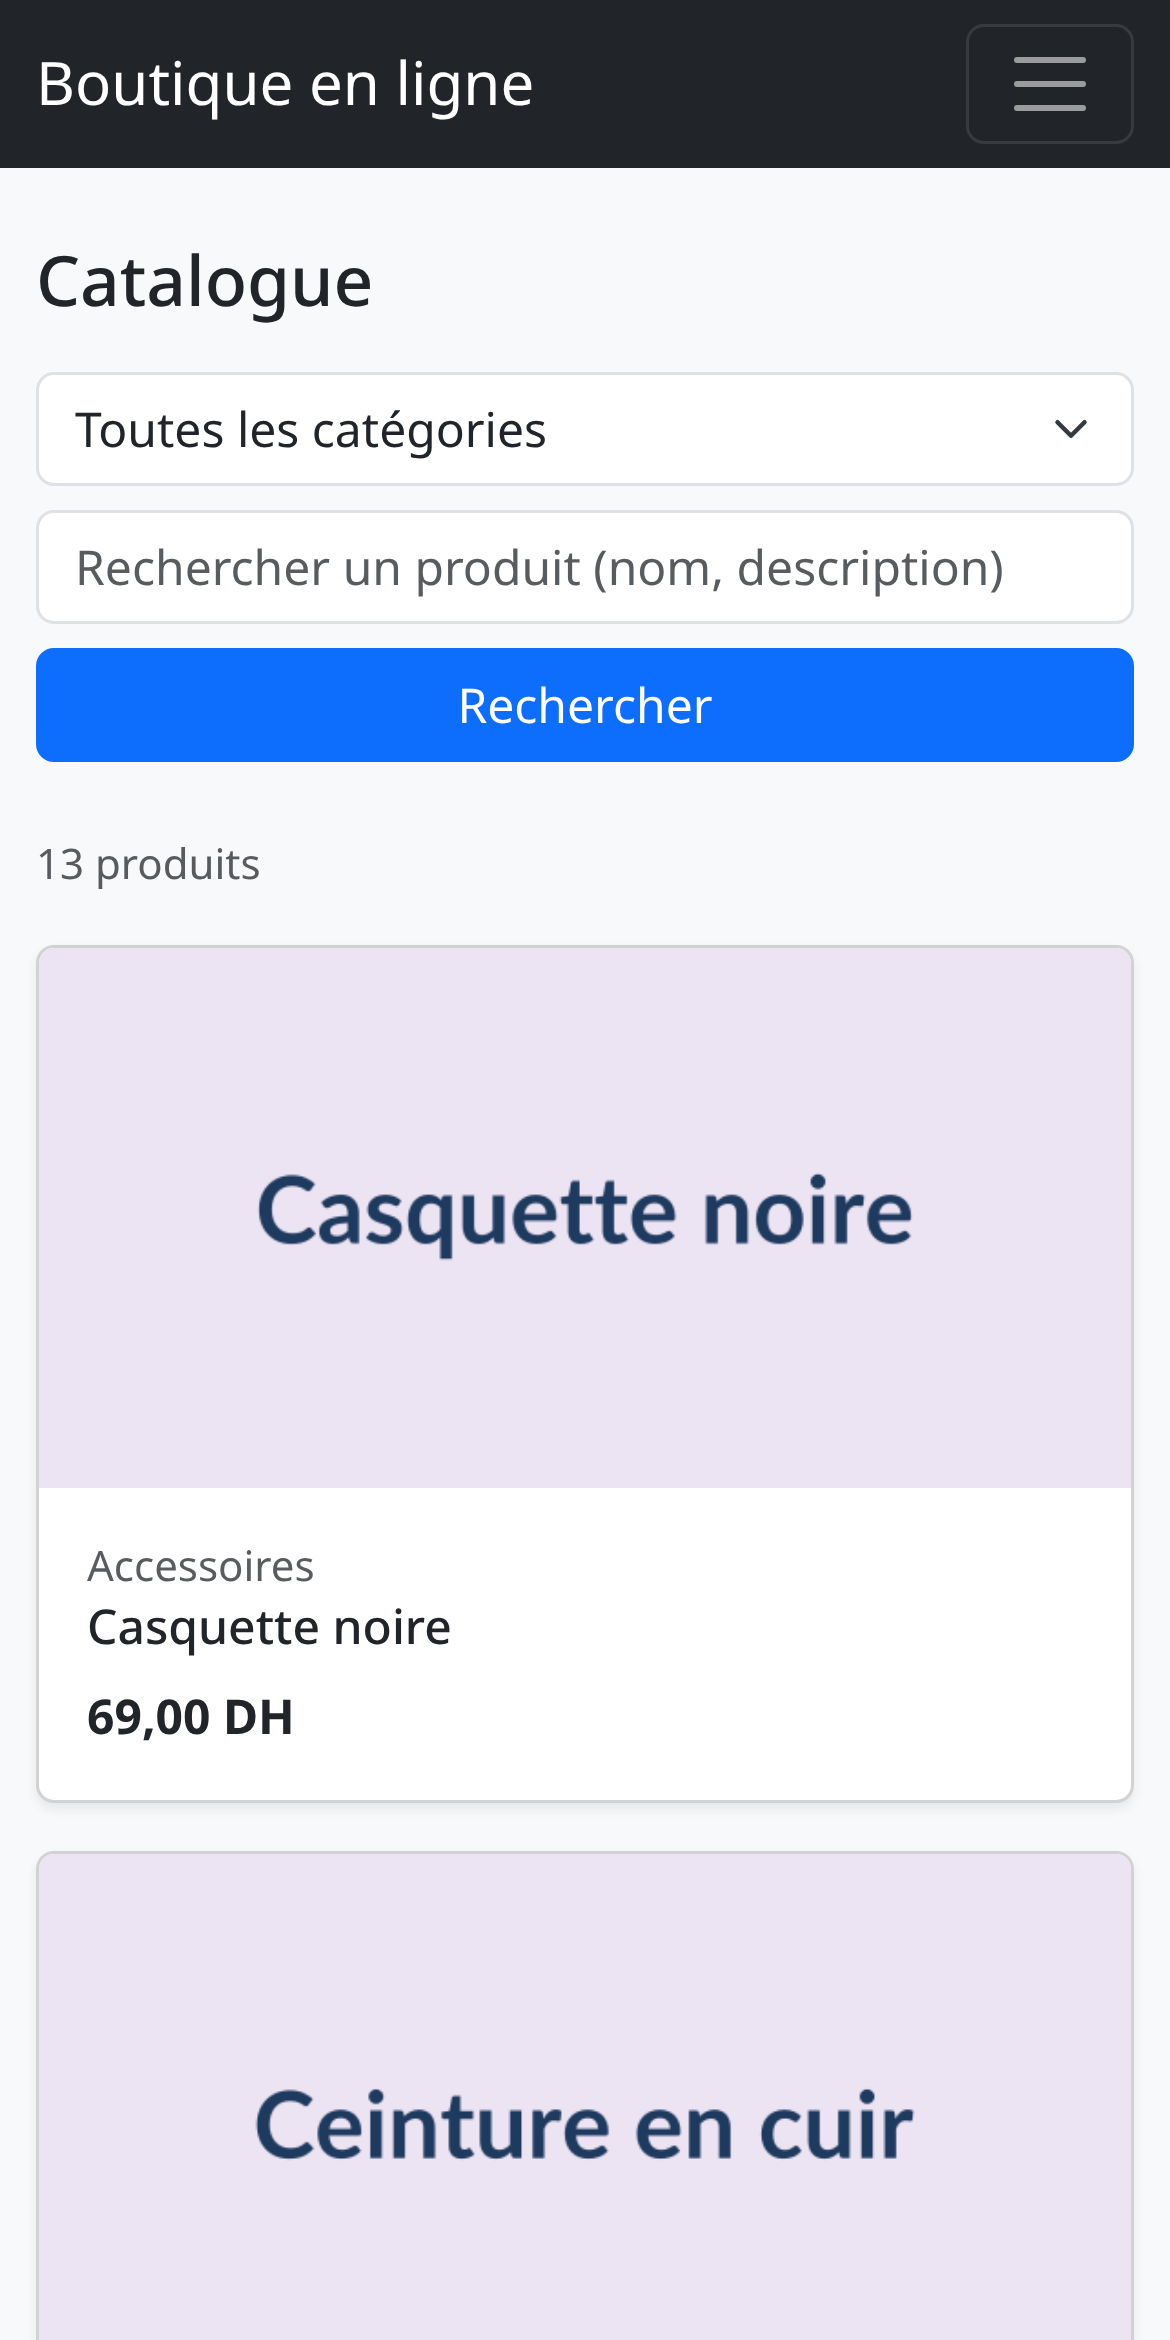
\includegraphics[height=0.5\textheight]{captures/mobile-catalogue.png}\hspace{1cm}
  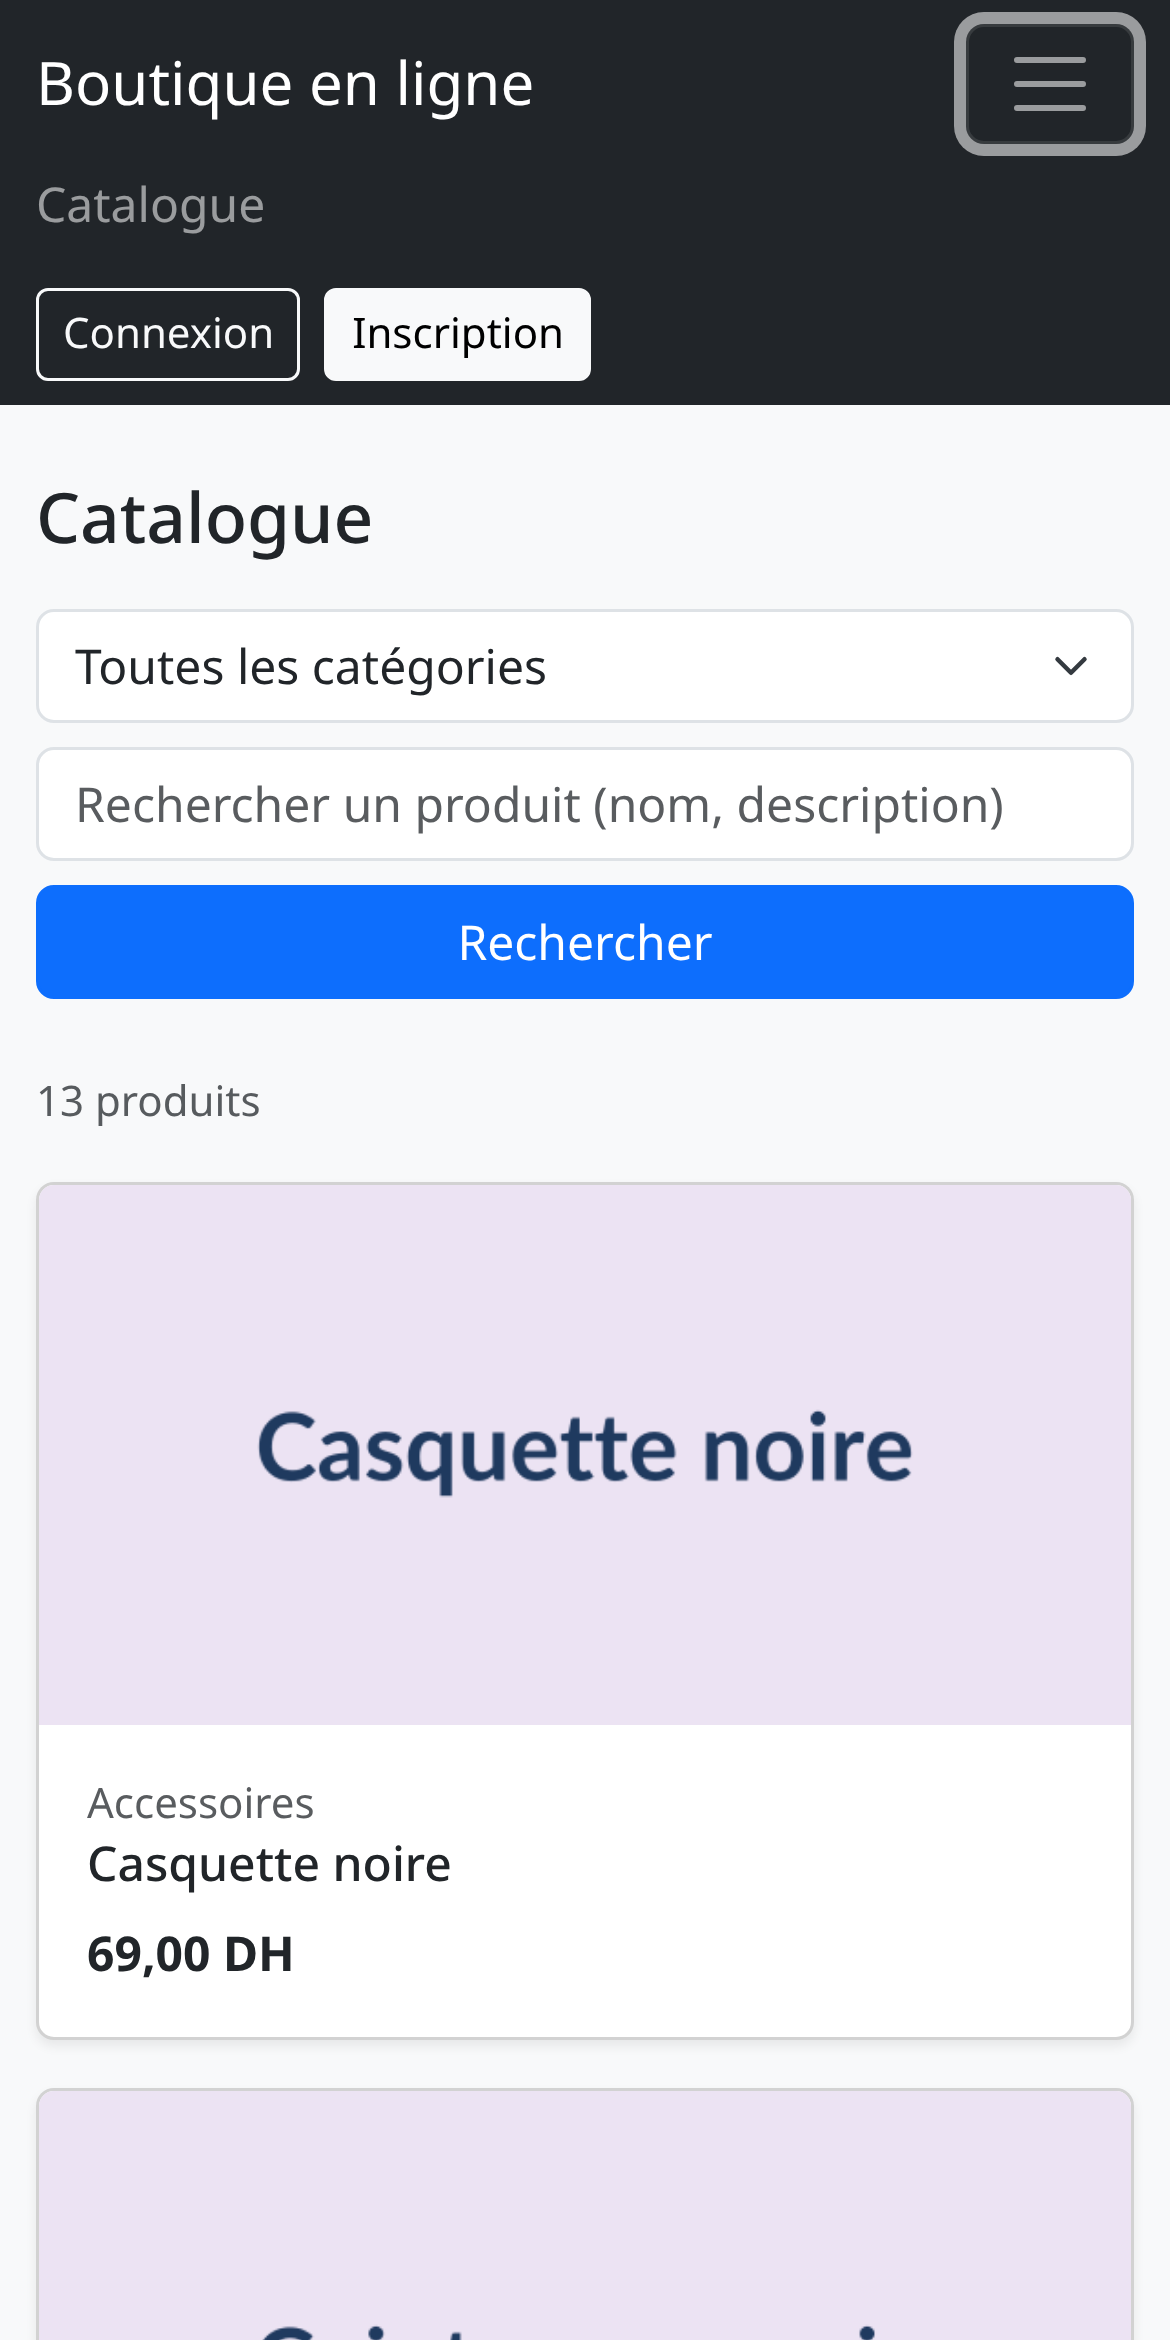
\includegraphics[height=0.5\textheight]{captures/mobile-menu.png}
  \caption{Affichage mobile : barre de navigation repliée, puis dépliée (BNF08)}
\end{figure}

\section{Base de données}

Tables générées par Hibernate (\code{hbm2ddl.auto = update}) à partir des entités, et structure de deux d'entre
elles, telles que les affiche le client \code{mysql} :

{\footnotesize
\begin{verbatim}
mysql> show tables;
+--------------------+
| Tables_in_boutique |
+--------------------+
| categorie          |
| commande           |
| ligne_commande     |
| produit            |
| utilisateur        |
+--------------------+

mysql> describe produit;
+---------------+---------------+------+-----+---------+----------------+
| Field         | Type          | Null | Key | Default | Extra          |
+---------------+---------------+------+-----+---------+----------------+
| id            | bigint        | NO   | PRI | NULL    | auto_increment |
| actif         | bit(1)        | NO   |     | NULL    |                |
| date_creation | datetime(6)   | NO   |     | NULL    |                |
| description   | varchar(2000) | YES  |     | NULL    |                |
| image_url     | varchar(500)  | YES  |     | NULL    |                |
| nom           | varchar(150)  | NO   |     | NULL    |                |
| prix          | decimal(10,2) | NO   |     | NULL    |                |
| stock         | int           | NO   |     | NULL    |                |
| categorie_id  | bigint        | NO   | MUL | NULL    |                |
+---------------+---------------+------+-----+---------+----------------+

mysql> describe ligne_commande;
+---------------+---------------+------+-----+---------+----------------+
| Field         | Type          | Null | Key | Default | Extra          |
+---------------+---------------+------+-----+---------+----------------+
| id            | bigint        | NO   | PRI | NULL    | auto_increment |
| prix_unitaire | decimal(10,2) | NO   |     | NULL    |                |
| quantite      | int           | NO   |     | NULL    |                |
| commande_id   | bigint        | NO   | MUL | NULL    |                |
| produit_id    | bigint        | NO   | MUL | NULL    |                |
+---------------+---------------+------+-----+---------+----------------+
\end{verbatim}
}

\chapter{Références}

\begin{itemize}
  \item Dépôt du projet : \url{https://github.com/unk-user/Boutique-JEE}
  \item Cahier des charges : \code{docs/cahier-des-charges.md}
  \item Diagrammes UML : \code{docs/uml/} (sources \code{.puml}, exports \code{.svg})
  \item Installation et déploiement : \code{README.md}
  \item Script du premier administrateur : \code{docs/sql/admin.sql}
\end{itemize}


\end{document}
